%% arara directives
% arara: xelatex
% arara: bibtex
% arara: xelatex
% arara: xelatex

%\documentclass{article} % One-column default
\documentclass[twocolumn, switch]{article} % Method A for two-column formatting

\usepackage{preprint}

%% Math packages
\usepackage{amsmath, amsthm, amssymb, amsfonts, algorithm2e, algpseudocode, graphicx, caption, subcaption, multirow}
\RestyleAlgo{ruled}
\graphicspath{ {./Pictures/} }
%% Bibliography options
\usepackage[numbers,square]{natbib}
\bibliographystyle{unsrtnat}
%\usepackage{natbib}
%\bibliographystyle{Geology}

%% General packages
\usepackage[utf8]{inputenc}	% allow utf-8 input
\usepackage[T1]{fontenc}	% use 8-bit T1 fonts
\usepackage{xcolor}		% colors for hyperlinks
\usepackage[colorlinks = true,
            linkcolor = purple,
            urlcolor  = blue,
            citecolor = cyan,
            anchorcolor = black]{hyperref}	% Color links to references, figures, etc.
\usepackage{booktabs} 		% professional-quality tables
\usepackage{nicefrac}		% compact symbols for 1/2, etc.
\usepackage{microtype}		% microtypography
\usepackage{lineno}		% Line numbers
\usepackage{float}			% Allows for figures within multicol
%\usepackage{multicol}		% Multiple columns (Method B)

\usepackage{lipsum}		%  Filler text

 %% Special figure caption options
\usepackage{newfloat}
\DeclareFloatingEnvironment[name={Supplementary Figure}]{suppfigure}
\usepackage{sidecap}
\sidecaptionvpos{figure}{c}

% Section title spacing  options
\usepackage{titlesec}
\titlespacing\section{0pt}{12pt plus 3pt minus 3pt}{1pt plus 1pt minus 1pt}
\titlespacing\subsection{0pt}{10pt plus 3pt minus 3pt}{1pt plus 1pt minus 1pt}
\titlespacing\subsubsection{0pt}{8pt plus 3pt minus 3pt}{1pt plus 1pt minus 1pt}

% ORCiD insertion
\usepackage{tikz,xcolor,hyperref}

\definecolor{lime}{HTML}{A6CE39}
\DeclareRobustCommand{\orcidicon}{
	
\begin{tikzpicture}
	\draw[lime, fill=lime] (0,0) 
	circle [radius=0.16] 
	node[white] {{\fontfamily{qag}\selectfont \tiny ID}};
	\draw[white, fill=white] (-0.0625,0.095) 
	circle [radius=0.007];
	\end{tikzpicture}
	\hspace{-2mm}
}
\foreach \x in {A, ..., Z}{\expandafter\xdef\csname orcid\x\endcsname{\noexpand\href{https://orcid.org/\csname orcidauthor\x\endcsname}
			{\noexpand\orcidicon}}
}
% Define the ORCID iD command for each author separately. Here done for two authors.
\newcommand{\orcidauthorA}{0000-0000-0000-0001}
\newcommand{\orcidauthorB}{0000-0000-0000-0002}
\newcommand{\orcidauthorC}{0000-0000-0000-0003}
\newcommand{\orcidauthorD}{0000-0000-0000-0004}

%%%%%%%%%%%%%%%%   Title   %%%%%%%%%%%%%%%%
\title{Parallel A* project}

% Add watermark with submission status
\usepackage{xwatermark}
% Left watermark
\newwatermark[firstpage,color=gray!60,angle=90,scale=0.32, xpos=-4.05in,ypos=0]{\href{https://doi.org/}{\color{gray}{Publication doi}}}
% Right watermark
\newwatermark[firstpage,color=gray!60,angle=90,scale=0.32, xpos=3.9in,ypos=0]{\href{https://doi.org/}{\color{gray}{Preprint doi}}}
% Bottom watermark
\newwatermark[firstpage,color=gray!90,angle=0,scale=0.28, xpos=0in,ypos=-5in]{*correspondence: \texttt{email@institution.edu}}

%%%%%%%%%%%%%%%  Author list  %%%%%%%%%%%%%%%
\usepackage{authblk}
\renewcommand*{\Authfont}{\bfseries}
\author{Lorenzo Ippolito, Mattia Rosso, Fabio Mirto}


%%%%%%%%%%%%%%    Front matter    %%%%%%%%%%%%%%
\begin{document}

\twocolumn[ % Method A for two-column formatting
  \begin{@twocolumnfalse} % Method A for two-column formatting
  
\maketitle

\begin{abstract}
  ...Here the abstract...
\end{abstract}
%\keywords{First keyword \and Second keyword \and More} % (optional)
\vspace{0.35cm}

  \end{@twocolumnfalse} % Method A for two-column formatting
] % Method A for two-column formatting

%\begin{multicols}{2} % Method B for two-column formatting (doesn't play well with line numbers), comment out if using method A


%%%%%%%%%%%%%%%  Main text   %%%%%%%%%%%%%%%
% \linenumbers

%% %%%%%%%%%%%%%%%%%%%%%%% %%
%% CHAPTER 1: INTRODUCTION %%
%% %%%%%%%%%%%%%%%%%%%%%%% %%
\section{Introduction: about the A* algorithm}
A* is a graph-traversal and path-search algorithm. It is used in many contexts of computer science and 
not only. It can be considered as a general case of the Dijkstra algorithm and it achieves better performaces
with respect to it. It is a Greedy-best-first-search algorithm that uses an heuristic function to guide
itself. What it does is combining:
\begin{itemize}
  \item Dijkstra approach: favore nodes closed to the starting point(source)
  \item Greedy-best-first-search approach: favore nodes closed to the final point(destination)
\end{itemize}
Using the standard terminology we have:
\begin{itemize}
  \item $g(n)$: exact cost of moving from source to n
  \item $h(n)$: heuristic estimated cost of moving from a node n(source included) to the destination
  \item $f(n) = g(n) + h(n)$: in this way we are able to combine the actual cost with the estimated one
\end{itemize}
At each (main loop) iteration the node $n$ that has the minimum $f(n)$ is examinated.
\subsection{Heuristic design}
\paragraph{Premises} We are going to work with weighted oriented graph where $V$ is the set on nodes/vertices
and $E$ is the set of edges of the form $(x,y)$ to indicate that an oriented edge from $x$ to $y$ exists and it
has weight $cost(x, y)$.
\paragraph{Heuristic properties} 
The heurstic function represents the acutal core of the A* algorithm. It represents a prior-knowledge that
we have about the cost of the path from every node (source included) to the destination. 
\begin{itemize}
  \item If we have not this prior information($h(n) = 0 \;\forall n \in V$) we are turning the A* algorithm into
        Dijkstra (this is why A* can be considered as a more general case of Dijkstra algorithm) but we always
        have the guarantee of finding the shortest path. 
  \item Admissible Heuristic: if $h(n) < cost(n, dest) \;\forall n \in V$ (so the we never over-estimate the distance to
        get to the destination from a node $n$) A* will always find the shortest path and the heuristic
        function is called \textit{admissible}. The more inaccurate
        is the estimation the more nodes A* will need to expand (with the upper bound of expanding every
        nodes in the graph if $h(n) = 0$).
  \item Consistent Heuristic: if $h(x) \le cost(x, y) + h(y)$ for every edge $(x, y)$ (so the triangular
        inequality is satisfied) A* has the guarantee to find an optimal path without processing
        any node more than once. 
\end{itemize}
\paragraph{Corner cases} 
\begin{itemize}
  \item Dijkstra: As already discussed if $h(n)=0$ for every node in the graph A* turns into the Dijkstra algorithm.
  \item Ideal: We would obtain a perferct behaviour in case $h(n)$ is exactly equal to the cost of moving from $n$ to
  the destination (A* will only expand the nodes on the best path to get to the destination).
  \item Full greedy-best-first search: if $h(n) \gg g(n)$ than only $h(n)$ plays a role and A* turns into
        a completly greedy-best-first search algorithm.
\end{itemize}

%% %%%%%%%%%%%%%%%%%%%%%% %%
%% CHAPTER 2: APPLICATION %%
%% %%%%%%%%%%%%%%%%%%%%%% %%
\section{A* project application}
\paragraph{Problem definition} Given a wide range of fields where the A* algorithm can be applied we have choosed the one of
optimal path searching in geographical areas where the goal is to find the minimum distance path from a 
node source to a node destination.

\paragraph{Notation} We work with a weighted oriented graph $G$ that is made of nodes $n \in V$ that represents
road-realated points of interest and edges $(x,y) \in E$ represent the unidirectional connections among these points.
Each edge $(x, y)$ is associated to a weight that is the great-circle distance between $x$ and $y$ measured
in meters.
\paragraph{Benchmark} We will exploit the DIMACS benchmark to make robust estimates of the designed algortithms.
Starting from the FIPS system format files provided we have adopted them (as better explained in section ...) to provide
to the algorithms a file containing information structured as:
\begin{itemize}
  \item Nodes: each node $n$ is defined as $(index, longitude, latitude)$ where $index$ is a natural progressive
        number starting from $0$ used to univocally identify the node and $(longitude, latitude)$ are the geographical
        coordinates of the node.
  \item Edges: each edge $(x, y)$ is defined as $(x, y, weight)$ that represent a unidirectional connection
        from $x$ to $y$ (a road) with length $weight$ (great-circle distance from $x$ to $y$).
\end{itemize}
\subsection{Heuristic function: the great-circle distance}
As previoulsly discussed the A* needs an admssible and consistent heuristic to properly work and this
function is tipically problem-specific. Given the type of problem we are going to apply A* to we are going
to use a measure of geographical distance that extends the concept of heuclidean distance between two points:
the great circle distance (that is the shortest distance over the earth surface measured along the
earth surface itself).
\begin{figure}[ht!]
  \centering
  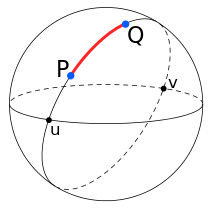
\includegraphics[width=0.5\linewidth]{haversine.png}
  \caption{Great circle distance from P to Q}
  \label{haversine}
\end{figure}
We will employee the Haversine formula to compute the distance from node $(\phi_1,\lambda_1)$
and $(\phi_1,\lambda_1)$ where $\phi$ is the latitude and $\lambda$ is the longitude:
\begin{center}
  $d = R \cdot c$\\
  where $c = 2 \cdot atan2(\sqrt{a},\sqrt{1-a})$\\
  $a = sin^2\Big({\frac{\Delta \phi}{2}}\Big) + cos(\phi_1) \cdot cos(\phi_2) \cdot sin^2\Big({\frac{\Delta \lambda}{2}}\Big)$
  \\$R$ is the earth radius that we have fixed to $R=6.371km$
\end{center}

%% %%%%%%%%%%%%%%%%%%%%%% %%
%% CHAPTER 1: INPUT GRAPH %%
%% %%%%%%%%%%%%%%%%%%%%%% %%
\section{Graph file input}
\paragraph{File input format} 
Now we start discussing the A* alogorithm implementation and to do that we need to specify which 
types of files we will need to provide to the algorithm to load the graph of interest. Each file has 
the format:
\begin{itemize}
    \item First line: the number of nodes $N[int]$
    \item N following lines: nodes appearing as $(index[int], longitude[double], latidue[double])$
    \item E following lines (with E unknown): edges appearing as $(x[int], y[int], weight[double])$
\end{itemize}
\paragraph{Random test graph} We have tested the designed algorithms also a random generated graph that
is build starting from: 
\begin{itemize}
  \item Which path we want to find: given the couple (source, destination) it is generated a graph of
        $max(source, destination) + 1$ nodes.
  \item How many paths at most have to be generated from source to destination
  \item The maximum length of these paths (that will be randomly chosen for each path)
\end{itemize}
In this way we have ad-hoc files to stress the algorithm having the guarantee that more than one path
exists from source to destination (other more standart approach exist for random graph generation but we
have implemented this custom one for this reason). To be consistent with benchmark files also these
random graphs represents geographic points with longitude and latitude.
\paragraph{DIMACS benchmark} 
The benchmark files we have used come from the DIMACS benchmark. Here each geographic map is described by:
\begin{itemize}
  \item \textit{.co} file: a file containing the coordinates of the nodes following the FIPS system notation
  \item \textit{.gr} file: a file containing the edges and the relative weight(distance) expressed in meters
\end{itemize}
The generation of a file consistent with the format described above happens by merging these files 
into a new one (in binary format). One of the challenge we are going to undertake is the one of
parallelizing the reading of these huge files (that we will show having an high impact in terms of
execution time over the overall A* algorithm).
\paragraph{Test paths}
To analyze the performance of the different versions of A* algorithms we have used these paths:
\begin{table}[ht!]
	\caption{Test paths for A*}
	\centering
	\begin{tabular}{ |l|l|l|l| }
		\hline
		Nodes & Edges & Source & Dest \\ 
    \hline
		\multicolumn{4}{ |c| }{\bf{Random map}} \\
		\hline
		\multirow{1}{*}{}
		 101& - & 0 & 100\\
		\hline
		\multicolumn{4}{ |c| }{\bf{California(BAY) map}} \\
		\hline
		\multirow{1}{*}{}
		321270& 800172 & 321269 & 263446\\
		\hline
		\multicolumn{4}{ |c| }{\bf{Florida(FLA) map}} \\
		\hline
		\multirow{1}{*}{}
		1070376& 2712798 & 0 & 103585\\
		\hline
	\end{tabular}
\end{table}
The paths on benchmark graphs BAY and FLA have been choosen ad-hoc to traverse the entire map with
a reasonable long path.
\begin{figure}[ht!]
  \centering
  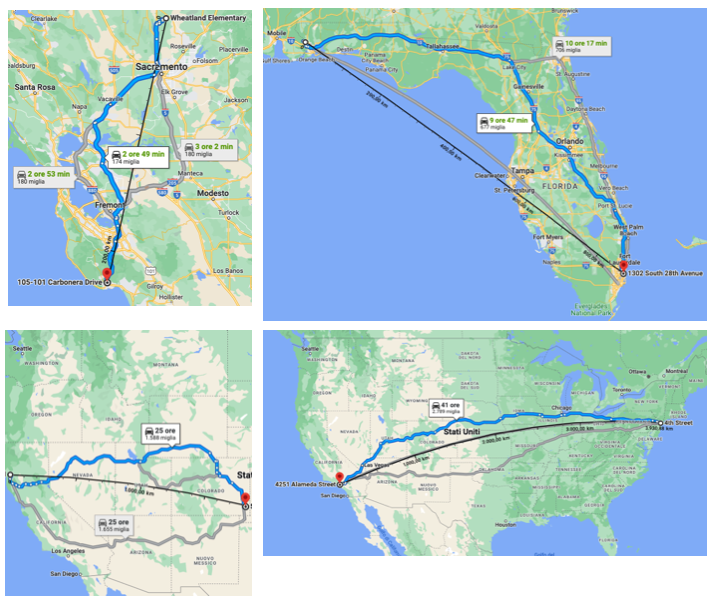
\includegraphics[width=0.75\linewidth]{google_maps.png}
  \caption{Test paths on BAY(left) and FLA(right)}
  \label{testpaths}
\end{figure}

%% %%%%%%%%%%%%%%%%%%%%%%%% %%
%% CHAPTER 1: A* SEQUENTIAL %%
%% %%%%%%%%%%%%%%%%%%%%%%%% %%
\section{Sequential A* Algorithm}
Sequential A* algorithm is the one we will start with to see how the algorithm works and performs.
The first step consists of a pre-computation of:
\begin{itemize}
  \item The heurstic $h(n)$ for each node (by defintion the $h(dest)$ will
        be 0) computed through the Haversine formula. We thus keep a global data
        structure \texttt{h} to do this.
  \item The initial values of $f(n)$ and $g(n)$ that will be set to $DOUBLE\_MAX$ for each
        node except for the source node that will have $f(source) = h(source)$ because 
        $g(soruce)$ is clearly $0$. We thus keep global data structures \texttt{f} and \texttt{g} to do this. 
        $f(source) = g(source) + h(source) = 0 + h(source) = h(source)$.
\end{itemize}
We will also need two additional global data structures:
\begin{itemize}
  \item The global \textit{costToCome} table (where \texttt{costToCome[i]} contains the current
        best cost to reach node \texttt{i}) that is initialized
        to $DOUBLE\_MAX$.
  \item The global \textit{parentVertex} table (where \texttt{parentVertex[i]} contains the
        parent node of node \texttt{i} according to the current best path found to reach
        the destination) that is initialized with $-1$.
\end{itemize}
The outer loop is based on the nodes extraction from a \textit{open set}, the one containing
the nodes that have still to be explored (it is implemented as a Priory Queue where the priority
is associated to the $f(n)$ of the nodes). At each iteration the node $a$ with minimum $f(a)$ is
extracted from the \textit{open set} and its neighbors are expanded: the inner loop is repeated once for each neighbor $b$ of the
extracted node $a$($b$ is neighbor of $a$ if the edge $(a, b)$ exists). A tentative score is computed
for each node $b$ as $g(b) = g(a) + weight(a, b)$. If $g(b)$ is less than current \texttt{g[b]} these data structures
are updated: 
\begin{flushleft}
  \texttt{g[b] = g[a] + weight(a, b)}\\
  \texttt{costToCome[b] = g[b]}\\
  \texttt{parentVertex[b] = a}\\
  \texttt{f[b] = g[b] + h[b]}
\end{flushleft}
The final step of this inner loop is checking wheter the node $b$ has already been added to the 
\textit{open set} or not. In case the \textit{open set} doesn't contain it we add it (with priority
$f(n)$ just computed).
Since the heuristic function we have chosen is both admissible and consistent we have the guarantee 
that the first time a node is extracted from the \textit{open set} we have found a best path to it (this
is why when the destination node is extracted we can terminate having found the best path). So despite
the node may be added to the \textit{open set} more than once (when discovered as a neighbor of different nodes)
it will be only expanded once.
\subsection{Pseudocode}
\SetKwComment{Comment}{/* }{ */}
\begin{algorithm}[ht!] 
\caption{Sequential A*}\label{alg:two}
\KwData{Graph G(V,E), Source s, Destination d, Heurstic h}
\KwResult{Best path from Source to Destination and relative cost}
$g[i] \gets DOUBLE\_MAX \;\forall i \in V$\;
$f[i] \gets DOUBLE\_MAX \;\forall i \in V$\;
$h[i] \gets h(i, d) \; \forall i \in V$\;
$costToCome[i] \gets 1 \; \forall i \in V$\;
$parentVertex[i] \gets 1 \; \forall i \in V$\;
$f[s] \gets h[s]$\;
$g[s] \gets 0$\;
$openSet := \{(s, f[s])\}$\;
\While{$!openSet.EMPTY()$}{
  $a \gets openSet.POP()$\;
  \If{$a == d$}{
    $pathFound \gets true$\;
    reconstructPath()\;
  }
  %\Comment*[r]{Inner loop}
  \ForEach{neighbor $b$ of $a$}{
    $wt \gets weight(a, b)$\;
    $tentativeScore \gets g[a] + wt$\;
    \If{$tentativeScore$ is less than $g[b]$}{
      $parentVertex[b] \gets a$\;
      $costToCome[b] \gets wt$\;
      $g[b] \gets tentativeScore$\;
      $f[b] \gets g[b] + h[b]$\;
      \If{$!openSet.CONTAINS(b)$}{
        $openSet.PUSH((b, f[b]))$\;
      }
    }
  }
}
\end{algorithm}

\subsection{Results}
We are now going to run the sequential A* algorithm.
\begin{table}[]
  \caption{Sequential algorithms performance}
  \begin{tabular}{|l|l|l|l|l|l|}
  \hline
  \textbf{}    & \textbf{File Size} & \textbf{Reading} & \textbf{A*} & \textbf{Total} & \textbf{\begin{tabular}[c]{@{}l@{}}Reading \\ Impact\end{tabular}} \\ \hline
  \textbf{RND} & 2876B              & 0.0011s          & 0.0862s     & 1.1714s        & 1.2872\%                                                           \\ \hline
  \textbf{BAY} & 20.51MB            & 0.9365s          & 0.2349s     & 1.1714s        & 79.9477\%                                                          \\ \hline
  \textbf{FLA} & 69.09MB            & 3.0728s          & 0.5893s     & 3.6621s        & 83.9075\%                                                          \\ \hline
  \end{tabular}
\end{table}
We can realize that (despite for the random graph that is too small to appreciate this result) the 
reading time has a very high impact on the overall execution time of the algorithm and in section 6
we will investigate three different techniques for parallelizing the reading of the file. 
\section{A* and Dijkstra: a comparison}
As already mentioned the Dijkstra algorithm can be considered as a particular case of A* where we
don't any prior knowledge about the distances of the nodes (heuristic $h(n) = 0 \;\forall n \in V$).
We have also seen that the more precise is the heuristic function we provide the less nodes the algorithm
will expand to get to the destination obtaining the best path. To investigate this point we have run
Dijkstra algorithm on the same graph (here we only consider BAY and FLA) comparing the number of 
expanded nodes by the two algorithms:

\begin{table}[ht!]
  \caption{Expanded nodes vs total nodes for Dijkstra and A*}
  \begin{tabular}{|l|l|l|}
  \hline
  \textbf{Expanded nodes} & \textbf{Dijkstra} & \textbf{Sequential A*}       \\ \hline
  \textbf{RND}            & 15 of 101         & 13 of 101         \\ \hline
  \textbf{BAY}            & 318725 of 321270  & 156950 of 321270  \\ \hline
  \textbf{FLA}            & 996956 of 1070376 & 591926 of 1070376 \\ \hline
  \end{tabular}
\end{table}

The number of expanded nodes is clearly much higher when Dijkstra algorithm is used and the picture
\ref{astardijkstra} cleary show in \textcolor{blue}{blue} the nodes expanded by the sequntial A* algorithm
while the \textcolor{red}{red} show the nodes expanded by the Dijkstra algorithm. In the BAY map Dijkstra
expands $50\%$ nodes more than A* while in FLA it is less evident since Dijkstra expands $38\%$ of nodes
more than A*.
\begin{figure}[ht!]
  \centering
  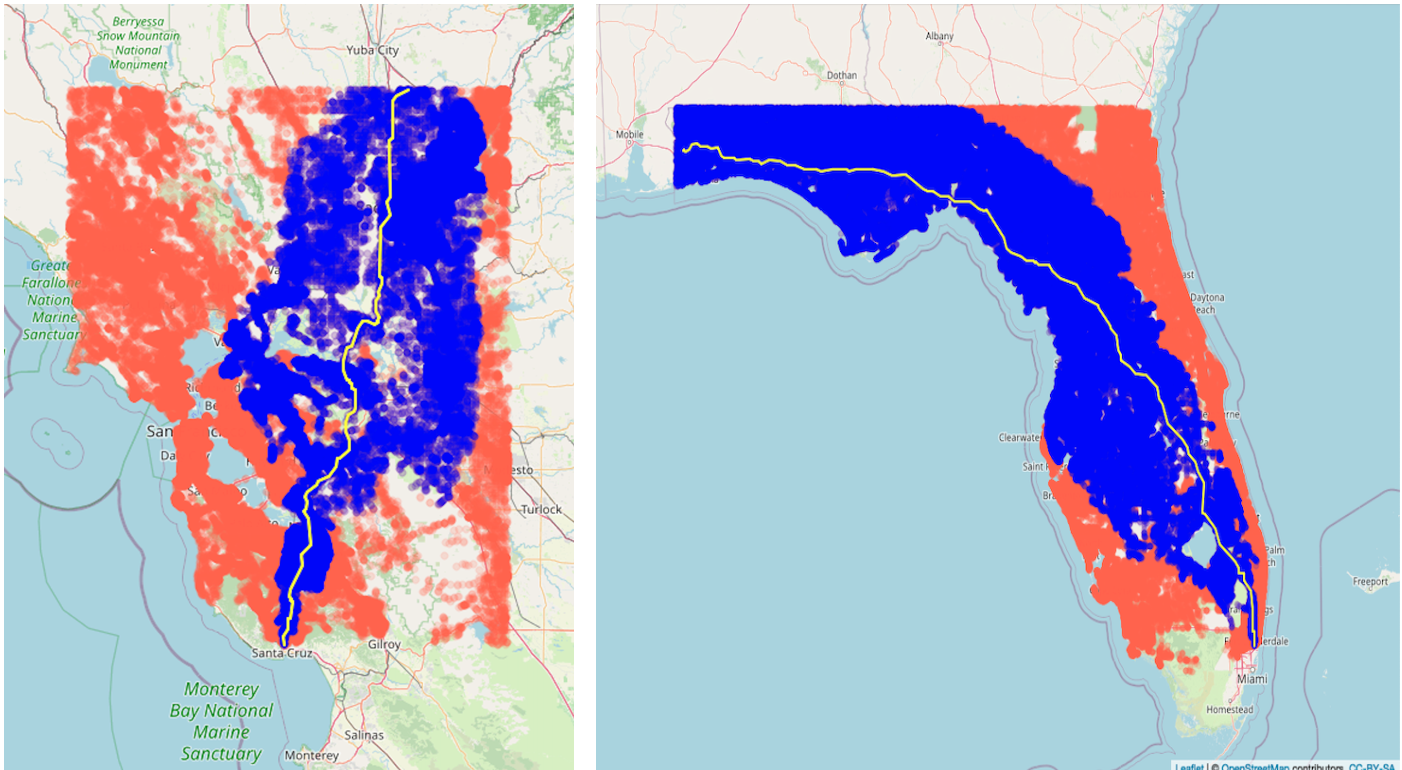
\includegraphics[width=1\linewidth]{dijkstra_astar.png}
  \caption{Test paths on BAY(left) and FLA(right)}
  \label{astardijkstra}
\end{figure}

\section{Parallel reading of the input file}
As we have seen in section 5 the time spent by the algorithm to read the input graph
(the input binary file) used by the A* algorithm is very high w.r.t. the total
amount of time spent. This is the reason why we have decided to inspect three techniques of
parallelization of the reading phase to speed it up. The input file, as already discussed,
is divided in two different sections (nodes and edges) so, in general, we need to take care of which
section a given thread is working on because different data structures of the graph need to
be loaded in the two sections (the symbol table when reading a \textit{node line} and the linked list when
reading a \textit{edge line}).
\subsection{Parallel Read: approach 1}
In this first approach we have implemeted a solution on which:
\begin{itemize}
  \item $N$ threads runs freely to read the entire file
  \item Only one file descriptor is shared among all the threads (this means that
        when thread $t_i$ performs a \texttt{read} opearation all the other threads 
        are waiting for it to finish)
\end{itemize}
This is the most trivial solution that can be adopted and the drawback is the really high
resource contention that exists among all the threads (when N threads whant to access line
$k$ of the file only $1$ can do it and others $N-1$ wait). The advantage is that the file
will be read \textit{sequentially} but in a multithread fashion (line $k$ of the file
is always read before line $k+1$) and this results in a easier implementation.
\paragraph{Results on BAY}
\begin{figure}[ht!]
  \centering
  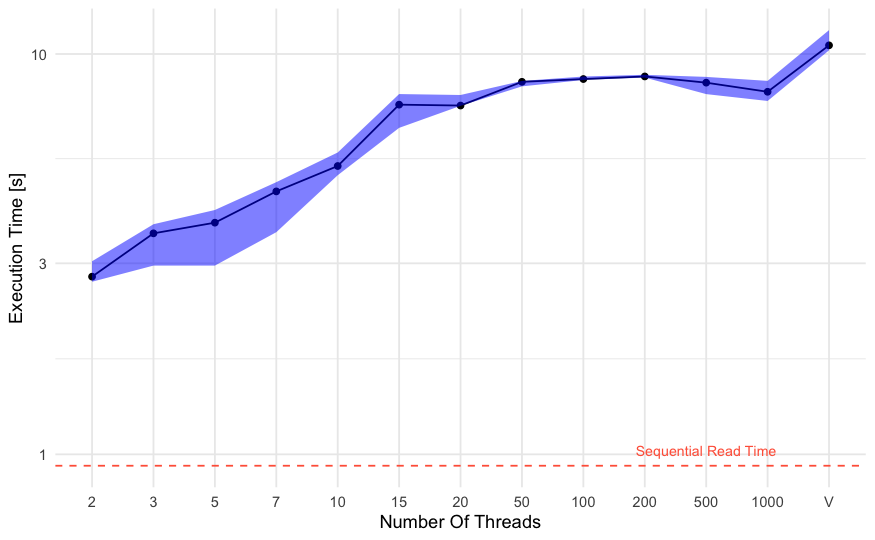
\includegraphics[width=1\linewidth]{par_read_1_time.png}
  \caption{Performance of approach 1 for different number of threads}
  \label{parread1time}
\end{figure}
\subsection{Parallel Read: approach 2}
(Explanation)
\paragraph{Results on BAY}
\begin{figure}[ht!]
  \centering
  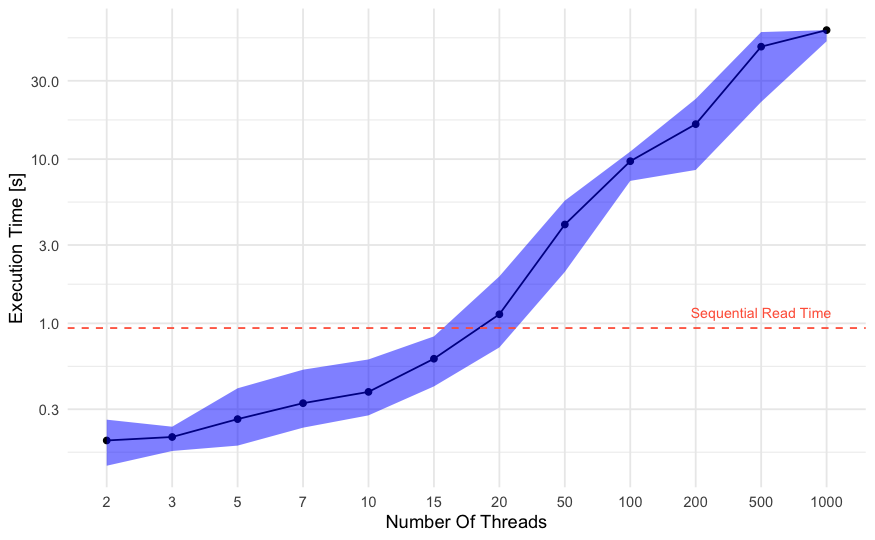
\includegraphics[width=1\linewidth]{par_read_2_time.png}
  \caption{Performance of approach 2 for different number of threads}
  \label{parread2time}
\end{figure}
\subsection{Parallel Read: approach 3}
This is the approach that generalize the first one by:
\begin{itemize}
  \item Letting threads differentiate among \textit{nodes section} and 
        \textit{edges section} to be able to read them togheter.
  \item Using a $(NP, NT)$ mechanism to read each section of the input file (where
        $NP$ is the number of partitions the section is divided in and $NT$ is the number
        of threads that have to read all the partitions).
\end{itemize}
\paragraph{The $(NP, NT)$ mechanism}
We need to provide as input:
\begin{itemize}
  \item $NP-nodes$: the number of partitions of the \textit{nodes section}
  \item $NP-edges$: the number of partitions of the \textit{edges section}
  \item $NT-nodes$: the number of threads that have to read the \textit{nodes section}
  \item $NT-edges$: the number of threads that have to read the \textit{edges section}
\end{itemize}
If the number of threads is equal to the number of partitions we have a simpler mechanism in
which each thread will read only one partition and then terminates.
As we can see in the example in figure \ref{parread3} threads will iterate over the partitions
of the sections that have been statically allocated to them. This means that there is not a real
contention of the reading phase since the partions are not overlapping and
each partition will be read by one and only one thread (actually, the
loading of the graph data structures after reading each line must be done in mutual exclusion so we will need a lock
both for the \textit{nodes-threads} and for the \textit{edges-threads}).
\begin{figure}[ht!]
  \centering
  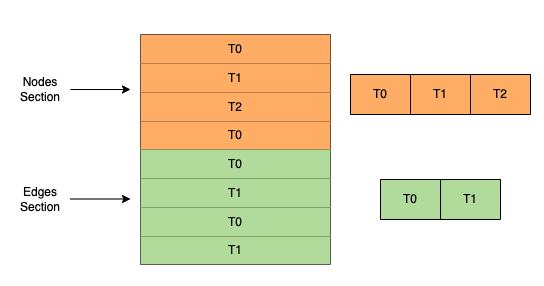
\includegraphics[width=1\linewidth]{par_read_3.png}
  \caption{Example of parallel read - approach 3}
  \label{parread3}
\end{figure}
Each thread terminates when it has no more partitions to read.\\
\paragraph{Results on BAY}
\begin{figure}[ht!]
  \centering
  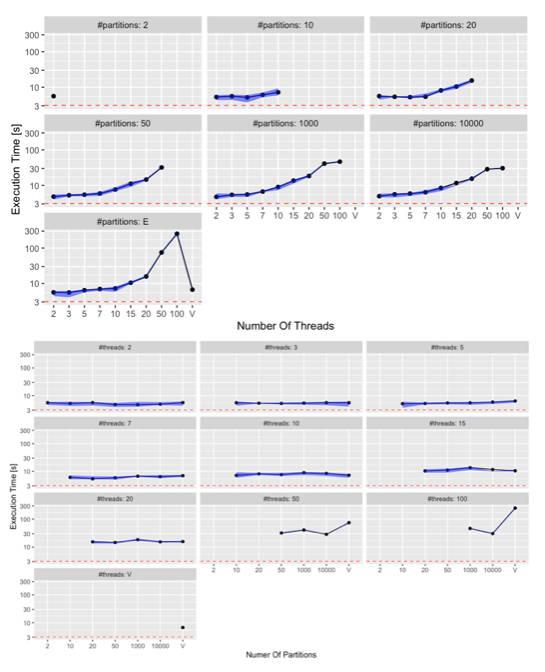
\includegraphics[width=1\linewidth]{par_read_3_time.png}
  \caption{Performance of approach 3 for different number of threads and partitions}
  \label{parread3time}
\end{figure}
We can realize from figure \ref{parread3time} that the number of partitions (setted equal
both for \textit{nodes section} and \textit{edges section}) has not a high impact.
What has an interesting impact is the number of threads. With a small number we are able
to reduce the reading time w.r.t the sequential approach while when increasing the 
number of threads results in too much overhead with consequent performance degradation.
\subsection{Final results}
\begin{figure}[ht!]
  \centering
  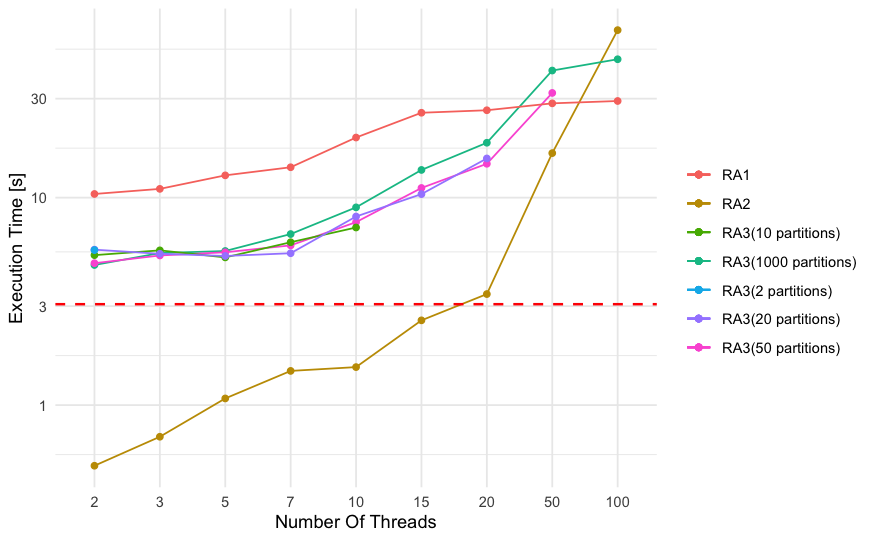
\includegraphics[width=1\linewidth]{par_read_all_time.png}
  \caption{RA(Read Approach) 1,2,3 compared with sequential reading}
  \label{parreadalltime}
\end{figure}
For the sake of completeness we have also test the most promising reading approaches
on FLA graph to check if they still perform well

\section{Parallel A*: two examinated approaches}
(Explanation)
\subsection{First Attempt In Parallelizing A*}
(Explanation + Pseudocode?)
\subsection{HDA*}
(Introduction + map with colored points)
\subsubsection{Message Passing Model}
(Explanation + Pseudocode?)
\subsubsection{Shared Address Space Model}
\paragraph{Barrier(SAS-B)}
(Explanation + Pseudocode?)
\paragraph{Barrier(SAS-SF)}
(Explanation + Pseudocode?)
\subsection{Results}
(Plots with the comparison of all the models with sequential A* on
random, BAY, FLA)

\section{Complete Results}
(Tables with numbers)

\section{Final Considerations}
(Comments)

\section{DIMACS Benchmark}
(More detailed explanation of the input format of the benchmarks)

\section{Future Works}
(Possible improvements)




%%%%%%%%%%%% Supplementary Methods %%%%%%%%%%%%
%\footnotesize
%\section*{Methods}

%%%%%%%%%%%%% Acknowledgements %%%%%%%%%%%%%
%\footnotesize
%\section*{Acknowledgements}

%%%%%%%%%%%%%%   Bibliography   %%%%%%%%%%%%%%
\normalsize
\bibliography{references}

%%%%%%%%%%%%  Supplementary Figures  %%%%%%%%%%%%
%\clearpage

%%%%%%%%%%%%%%%%   End   %%%%%%%%%%%%%%%%
%\end{multicols}  % Method B for two-column formatting (doesn't play well with line numbers), comment out if using method A
\end{document}